% !TEX program = pdflatex
% KAIROS --- Kinetic Analysis of Instantaneous RNA Output by Sequencing
% Colloquium, East Texas A&M University, 16 Apr 2026
% Build:  pdflatex kairos.tex  (2x for refs)

\documentclass[aspectratio=169,11pt]{beamer}
\usetheme{default}
\usecolortheme{default}
\setbeamertemplate{navigation symbols}{}

% --- Palette ------------------------------------------------------------
\definecolor{KNavy}{HTML}{0B1E3F}
\definecolor{KNavyDark}{HTML}{06142C}
\definecolor{KNavyLight}{HTML}{152A4E}
\definecolor{KGold}{HTML}{D4A017}
\definecolor{KGoldSoft}{HTML}{E6B422}
\definecolor{KCream}{HTML}{F3E9C6}
\definecolor{KSky}{HTML}{7FB5E6}
\definecolor{KRule}{HTML}{6B5215}
\definecolor{KWhite}{HTML}{F2F4F8}
\definecolor{KMuted}{HTML}{A9B3C2}

% --- Packages -----------------------------------------------------------
\usepackage{amsmath,amssymb,amsthm,mathtools}
\usepackage{graphicx}
\usepackage{tikz}
\usepackage{pgfplots}
\pgfplotsset{compat=1.18}
\usetikzlibrary{arrows.meta,positioning,calc,decorations.pathmorphing,%
                decorations.markings,shapes.geometric,backgrounds}
\usepackage{booktabs}
\usepackage{hyperref}
\usepackage{xcolor}
\usepackage{array}
\usepackage{lmodern}
\usepackage[T1]{fontenc}
\usepackage{microtype}

\graphicspath{{figures/}}

% --- Global look --------------------------------------------------------
\setbeamercolor{background canvas}{bg=KNavy}
\setbeamercolor{normal text}{fg=KWhite,bg=KNavy}
\setbeamercolor{structure}{fg=KGold}
\setbeamercolor{alerted text}{fg=KGoldSoft}
\setbeamercolor{example text}{fg=KSky}
\setbeamercolor{itemize item}{fg=KGold}
\setbeamercolor{itemize subitem}{fg=KSky}
\setbeamercolor{enumerate item}{fg=KGold}
\setbeamercolor{frametitle}{fg=KGold,bg=KNavy}
\setbeamerfont{frametitle}{series=\bfseries,size=\large}

% Frame title: gold text, thin gold rule, consistent left margin
\setbeamertemplate{frametitle}{%
  \nointerlineskip
  \vspace{0.8em}%
  \hspace{1.1em}{\insertframetitle}\par
  \vspace{0.2em}%
  \hspace{1.1em}{\color{KGold}\rule{0.92\paperwidth}{0.4pt}}%
  \vspace{0.4em}%
}

% Itemize bullets --- small, restrained
\setbeamertemplate{itemize item}{\color{KGold}\raisebox{0.25ex}{\scriptsize$\blacktriangleright$}}
\setbeamertemplate{itemize subitem}{\color{KSky}\scriptsize$\bullet$}
\setlength{\leftmargini}{1.3em}
\setbeamertemplate{itemize/enumerate body begin}{\small}

% Footer: hairline rule, subtle page counter
\setbeamertemplate{footline}{%
  \leavevmode%
  \vbox{%
    \hbox to \paperwidth{\hskip1.1em{\color{KRule}\rule{\dimexpr\paperwidth-2.2em\relax}{0.3pt}}\hskip1.1em}%
    \vskip0.35ex
    \hbox to \paperwidth{\hskip1.1em{\color{KMuted}\scriptsize KAIROS\,\textbullet\,Thornton\,\textbullet\,ETAMU Colloquium 2026}\hfil{\color{KMuted}\scriptsize\insertframenumber}\hskip1.1em}%
    \vskip0.7ex
  }%
}

% --- Helper macros ------------------------------------------------------
\newcommand{\smallKAIROS}{{\color{KGold}\bfseries KAIROS}}
\newcommand{\goldbf}[1]{{\color{KGold}\bfseries #1}}
\newcommand{\skyit}[1]{{\color{KSky}\itshape #1}}
\newcommand{\creambf}[1]{{\color{KCream}\bfseries #1}}

% A clean card: navy panel, hairline gold rule, short top accent stripe
\newcommand{\kcard}[4]{% {accent color}{number}{title}{body}
  \begin{tikzpicture}
    \node[rectangle,fill=KNavyLight,draw=KRule,line width=0.3pt,
          minimum width=4.6cm,minimum height=4.4cm,
          text width=4.1cm,align=left,anchor=north west,
          inner sep=10pt] (c) at (0,0) {%
      \parbox{4.1cm}{\vspace{0.1em}%
        {\color{#1}\rule{1.0cm}{1.8pt}}\\[0.6em]
        {\color{KSky}\scriptsize\bfseries #2}\hspace{0.4em}{\color{KGold}\small\bfseries #3}\\[0.55em]
        {\color{KWhite}\scriptsize\raggedright #4\par}%
      }%
    };
  \end{tikzpicture}%
}

% Section divider: big centered numeral
\newcommand{\bignum}[1]{%
  {\fontsize{140pt}{140pt}\selectfont\bfseries\color{KGold}#1}%
}

% ========================================================================
\begin{document}

% ---------- TITLE SLIDE ------------------------------------------------
{\setbeamercolor{background canvas}{bg=KNavy}
\begin{frame}[plain]
  \begin{tikzpicture}[remember picture,overlay]
    % thin top rule
    \draw[KGold,line width=0.4pt] ($(current page.north west)+(1.1,-1.0)$) --
                                   ($(current page.north east)+(-1.1,-1.0)$);
    % small overline label
    \node[anchor=north west,text=KCream,font=\footnotesize]
      at ($(current page.north west)+(1.1,-0.75)$) {East Texas A\&M University \textbullet\ Colloquium Presentation};
    \node[anchor=north east,text=KCream,font=\footnotesize]
      at ($(current page.north east)+(-1.1,-0.75)$) {April 16, 2026 \textbullet\ 4:00 PM \textbullet\ Room 127};

    % BIG KAIROS title, perfectly left-aligned
    \node[anchor=north west] at ($(current page.north west)+(1.1,-1.6)$) {%
      {\fontsize{72pt}{72pt}\selectfont\bfseries\color{KGold}KAIROS}%
    };
    % subtitle (italic cream), close under title
    \node[anchor=north west,text width=14cm]
      at ($(current page.north west)+(1.1,-3.5)$) {%
      {\color{KCream}\LARGE\itshape Kinetic Analysis of Instantaneous RNA Output by Sequencing}%
    };
    % divider rule
    \draw[KGold,line width=0.8pt] ($(current page.north west)+(1.1,-4.4)$) --
                                   ($(current page.north west)+(5.1,-4.4)$);

    % one-line tagline
    \node[anchor=north west,text width=14cm]
      at ($(current page.north west)+(1.1,-4.7)$) {%
      {\color{KMuted}\normalsize A position-resolved framework for RNA Polymerase II elongation kinetics.}%
    };

    % speaker block --- plain text, no card
    \node[anchor=south west,align=left]
      at ($(current page.south west)+(1.1,1.0)$) {%
      {\color{KGold}\bfseries\large Micah Thornton, PhD}\\[0.15em]
      {\color{KWhite}\small Assistant Professor of Mathematics}\\[0.05em]
      {\color{KCream}\small Texas Woman's University}%
    };

    % minimal DNA-helix motif, bottom-right, subdued
    \node[anchor=south east] at ($(current page.south east)+(-1.1,1.0)$) {%
      \begin{tikzpicture}[scale=0.85]
        \foreach \s in {0,...,48}{
          \pgfmathsetmacro{\x}{\s*0.13}
          \pgfmathsetmacro{\ya}{0.4*sin(\x*90)}
          \pgfmathsetmacro{\yb}{0.4*sin(\x*90+180)}
          \pgfmathsetmacro{\op}{0.20+0.55*\s/48}
          \fill[KSky,opacity=\op] (\x,\ya) circle (0.045);
          \fill[KGoldSoft,opacity=\op] (\x,\yb) circle (0.045);
        }
        \draw[->,KGold,line width=0.9pt,shorten >=1pt]
          (0,-0.85) -- (6.2,-0.85)
          node[midway,below=-1pt,text=KMuted,font=\scriptsize\itshape] {$5' \longrightarrow 3'$};
      \end{tikzpicture}%
    };

    % bottom hairline
    \draw[KRule,line width=0.3pt] ($(current page.south west)+(1.1,0.55)$) --
                                   ($(current page.south east)+(-1.1,0.55)$);
    \node[anchor=south,text=KMuted,font=\scriptsize]
      at ($(current page.south)+(0,0.22)$) {kairos \textbullet\ a moment of opportune time};
  \end{tikzpicture}
\end{frame}}

% ---------- AGENDA / THREE PILLARS -------------------------------------
\begin{frame}{Three pillars of \smallKAIROS}
  \vspace{0.4em}
  \begin{center}
  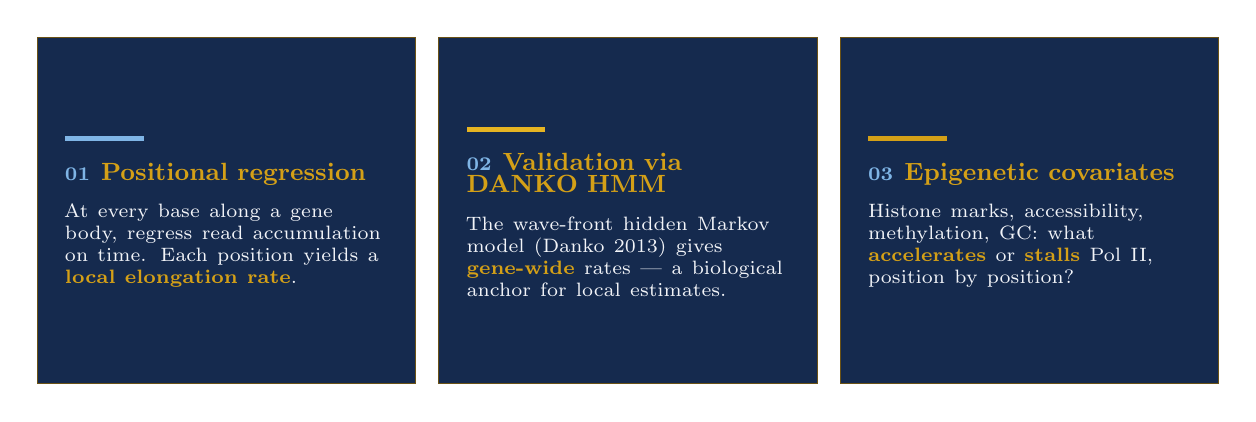
\begin{tikzpicture}[every node/.style={align=left}]
    \node[anchor=north west] at (0,0) {%
      \kcard{KSky}{01}{Positional regression}{%
        At every base along a gene body, regress read accumulation on time.
        Each position yields a \goldbf{local elongation rate}.
      }};
    \node[anchor=north west] at (5.1,0) {%
      \kcard{KGoldSoft}{02}{Validation via DANKO HMM}{%
        The wave-front hidden Markov model (Danko 2013) gives \goldbf{gene-wide}
        rates --- a biological anchor for local estimates.
      }};
    \node[anchor=north west] at (10.2,0) {%
      \kcard{KGold}{03}{Epigenetic covariates}{%
        Histone marks, accessibility, methylation, GC: what \goldbf{accelerates}
        or \goldbf{stalls} Pol II, position by position?
      }};
  \end{tikzpicture}
  \end{center}
  \vspace{1.2em}
  \begin{center}
    {\color{KCream}\itshape Transcription is not uniform.\ \ KAIROS treats each position as its own measurement.}
  \end{center}
\end{frame}

% ---------- THE QUESTION -----------------------------------------------
\begin{frame}{Why position-resolved speed?}
\begin{columns}[T,onlytextwidth]
\begin{column}{0.52\textwidth}
  \vspace{0.3em}
  {\color{KWhite}\small
  RNA Polymerase II does not elongate at constant velocity. Over a single
  gene body it \creambf{pauses}, \creambf{accelerates}, and
  \creambf{decelerates} under competing molecular forces:}
  \begin{itemize}
    \setlength{\itemsep}{0.2em}
    \item nucleosome positioning and histone marks
    \item DNA sequence context and GC skew
    \item cotranscriptional splicing signals
    \item DNA damage and R-loop formation
    \item exon / intron boundaries
  \end{itemize}
  \vspace{0.6em}
  {\color{KCream}\itshape\small
  A single gene-wide rate erases the kinetic landscape that makes
  transcription biologically informative.}
\end{column}
\begin{column}{0.46\textwidth}
  \centering
  \vspace{0.6em}
  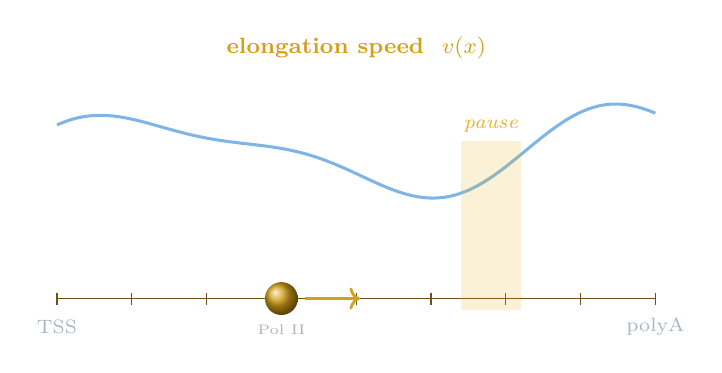
\begin{tikzpicture}[scale=0.95]
    % speed curve (top)
    \begin{scope}[yshift=1.3cm]
      \draw[KSky,line width=1.1pt,domain=0:8,smooth,samples=120,variable=\x]
        plot ({\x},{0.65 + 0.50*sin(\x*55+20) + 0.20*cos(\x*100)});
      \node[KGold,font=\footnotesize\bfseries] at (4,2.05) {elongation speed\ \ $v(x)$};
    \end{scope}
    % gene body
    \draw[KRule,line width=0.6pt] (0,0) -- (8,0);
    \foreach \x in {0,1,...,8}{\draw[KRule] (\x,-0.08) -- (\x,0.08);}
    \node[KMuted,font=\scriptsize] at (0,-0.38) {TSS};
    \node[KMuted,font=\scriptsize] at (8,-0.38) {polyA};
    % polymerase
    \shade[ball color=KGold] (3.0,0) circle (0.22);
    \node[KMuted,font=\tiny] at (3.0,-0.42) {Pol II};
    \draw[->,KGold,line width=1pt] (3.32,0) -- (4.05,0);
    % pause zone
    \fill[KGoldSoft,opacity=0.18] (5.4,-0.15) rectangle (6.2,2.1);
    \node[KGoldSoft,font=\scriptsize\itshape] at (5.8,2.3) {pause};
  \end{tikzpicture}
  \vspace{0.5em}

  {\color{KMuted}\scriptsize\itshape Speed varies along the gene body --- KAIROS recovers $v(x)$.}
\end{column}
\end{columns}
\end{frame}

% ---------- THE 1/v PRINCIPLE ------------------------------------------
\begin{frame}{The $1/v$ principle}
\begin{columns}[T,onlytextwidth]
\begin{column}{0.52\textwidth}
  \vspace{0.4em}
  {\color{KWhite}\small
  If Pol II moves through position $x$ at speed $v(x)$, the
  \goldbf{dwell-time} density is proportional to $1/v(x)$.}
  \medskip

  {\color{KWhite}\small
  In a nascent-RNA snapshot at elapsed time $t$:}
  \[
     \mathbb{E}\big[\,r(x,t)\,\big] \;\propto\; \frac{t}{v(x)}
     \qquad\Longrightarrow\qquad
     \widehat{v}(x) \;\propto\; \frac{t}{r(x,t)}.
  \]
  \medskip

  {\color{KCream}\itshape\small Slow regions look dark with reads; fast
  regions look sparse.\ \ The inverse relationship is the kinetic signature.}
\end{column}
\begin{column}{0.44\textwidth}
  \centering
  \vspace{0.4em}
  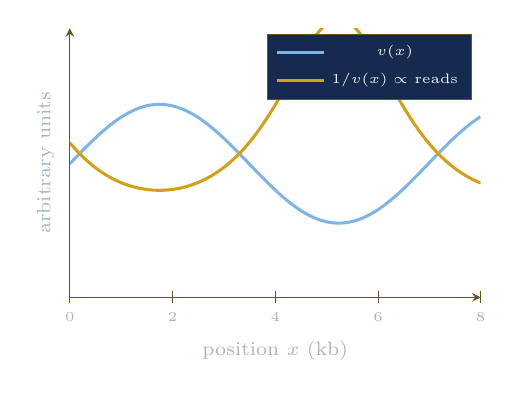
\begin{tikzpicture}
    \begin{axis}[
      width=6.8cm,height=5.0cm,
      axis lines=left,
      xlabel={\color{KMuted}\scriptsize position $x$ (kb)},
      ylabel={\color{KMuted}\scriptsize arbitrary units},
      axis line style={KRule,line width=0.4pt},
      tick style={KRule,line width=0.3pt},
      xtick={0,2,4,6,8}, ytick=\empty,
      xticklabel style={text=KMuted,font=\tiny},
      every axis label/.style={font=\scriptsize},
      enlargelimits=false,
      xmin=0,xmax=8,ymin=0,ymax=1.45,
      legend style={draw=KRule,fill=KNavyLight,text=KWhite,
                    font=\tiny,at={(0.98,0.98)},anchor=north east,
                    row sep=1pt},
      ]
      \addplot[KSky,line width=1.1pt,domain=0:8,samples=120]
        {0.72 + 0.32*sin(deg(x*0.9))};
      \addlegendentry{\color{KWhite}$v(x)$}
      \addplot[KGold,line width=1.1pt,domain=0:8,samples=120]
        {0.60/(0.72 + 0.32*sin(deg(x*0.9)))};
      \addlegendentry{\color{KWhite}$1/v(x) \propto$ reads}
    \end{axis}
  \end{tikzpicture}
\end{column}
\end{columns}
\end{frame}

% ---------- DATA --------------------------------------------------------
\begin{frame}{The data: GRO-seq time course (Danko et al., 2013)}
\begin{columns}[T,onlytextwidth]
\begin{column}{0.56\textwidth}
  \vspace{0.3em}
  \begin{itemize}
    \setlength{\itemsep}{0.35em}
    \item {\color{KWhite}\small\goldbf{Global Run-On sequencing} (GRO-seq) captures
          \emph{nascent} RNA on chromatin --- a snapshot of active Pol II.}
    \item {\color{KWhite}\small MCF-7 cells treated with 17$\beta$-estradiol; samples at
          $t \in \{0,\,10,\,25,\,40\}$ minutes.}
    \item {\color{KWhite}\small $\sim$2500 activated genes with clean signal used for downstream analysis.}
    \item {\color{KWhite}\small Anchor: \goldbf{DANKO HMM} gene-wide elongation rates (their Figure 4).}
  \end{itemize}
  \vspace{0.8em}
  {\color{KCream}\itshape\footnotesize
  Each gene becomes a trajectory on a space-time grid: rows are positions,
  columns are time points, cell $(x,t)$ is read density.}
\end{column}
\begin{column}{0.42\textwidth}
  \centering
  \vspace{0.8em}
  % Clean heatmap panels: deterministic gradient, no noise
  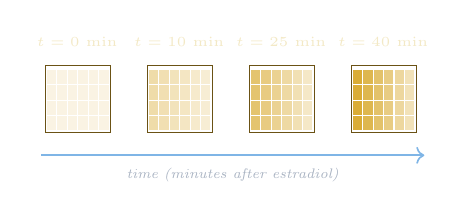
\begin{tikzpicture}[scale=0.70]
    \foreach \t [count=\i from 0] in {0,10,25,40}{
      \begin{scope}[xshift=\i*1.85cm]
        \node[KCream,font=\tiny,anchor=south] at (0.55,1.35) {$t=\t$ min};
        \foreach \y in {0,...,3}{
          \foreach \x in {0,...,5}{
            \pgfmathsetmacro{\op}{0.12 + 0.75*(\i/3)*(1 - 0.15*\x)}
            \fill[KGold,opacity=\op]
                 (\x*0.19,\y*0.28) rectangle (\x*0.19+0.17,\y*0.28+0.26);
          }
        }
        % small frame
        \draw[KRule,line width=0.2pt] (-0.03,-0.03) rectangle (1.16,1.18);
      \end{scope}
    }
    \draw[->,KSky,line width=0.6pt] (-0.1,-0.45) -- (6.85,-0.45)
      node[midway,below=1pt,text=KMuted,font=\tiny\itshape] {time (minutes after estradiol)};
  \end{tikzpicture}

  \vspace{1.4em}
  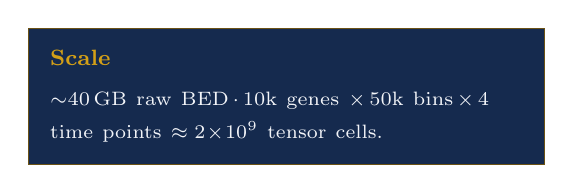
\begin{tikzpicture}
    \node[rectangle,draw=KRule,line width=0.3pt,fill=KNavyLight,
          inner sep=8pt,text width=6.0cm] {%
      {\color{KGold}\footnotesize\bfseries Scale}\\[0.25em]
      {\color{KWhite}\scriptsize $\sim$40\,GB raw BED\,$\cdot$\,10k genes
       $\times$\,50k bins\,$\times$\,4 time points
       $\approx 2\!\times\!10^9$ tensor cells.}%
    };
  \end{tikzpicture}
\end{column}
\end{columns}
\end{frame}

% ====================== SECTION DIVIDER 01 =============================
{\setbeamercolor{background canvas}{bg=KNavyDark}
\setbeamertemplate{footline}{}
\begin{frame}[plain]
  \begin{tikzpicture}[remember picture,overlay]
    % big numeral, left, vertically centered
    \node[anchor=center] at ($(current page.center)+(-4.5,0.4)$) {\bignum{01}};
    % vertical hairline separator
    \draw[KGold,line width=0.5pt]
      ($(current page.center)+(-2.5,2.2)$) -- ($(current page.center)+(-2.5,-2.2)$);
    % title + subtitle, right of rule
    \node[anchor=west,text width=9.5cm] at ($(current page.center)+(-2.1,1.0)$) {%
      {\color{KGold}\Huge\bfseries Positional Regression}\\[0.4em]
      {\color{KCream}\large\itshape Speed as a position-indexed slope.}%
    };
    \node[anchor=west,text width=9.5cm] at ($(current page.center)+(-2.1,-0.6)$) {%
      {\color{KMuted}\small
      For each position $x$ in a gene body, fit
      $r(x,t) = \alpha(x) + \beta(x)\,t + \varepsilon$\\[0.3em]
      and treat $\widehat\beta(x)$ as a velocity signature.}%
    };
  \end{tikzpicture}
\end{frame}}

% ---------- PILLAR 1: DETAIL -------------------------------------------
\begin{frame}{Positional regression: the estimator}
\begin{columns}[T,onlytextwidth]
\begin{column}{0.52\textwidth}
  \vspace{0.4em}
  {\color{KWhite}\small For gene $g$, position $x$, time points
  $t_i \in \{0,10,25,40\}$:}
  \[
    r_g(x,t_i) \;=\; \alpha_g(x) + \beta_g(x)\,t_i + \varepsilon_i .
  \]
  {\color{KWhite}\small The local slope $\widehat\beta_g(x)$ is the
  \goldbf{positional accumulation rate} (PAR). Since dwell time is
  $\propto 1/v(x)$:}
  \[
    \widehat v_g(x) \;\propto\; 1/\widehat\beta_g(x).
  \]
  \begin{itemize}
    \setlength{\itemsep}{0.25em}
    \item Robust M-estimator (Huber loss)
    \item Positions smoothed with a $\pm\,250$\,bp window
    \item Aggregated to gene level via algebraic diversity $Z_M$
  \end{itemize}
\end{column}
\begin{column}{0.44\textwidth}
  \centering
  \vspace{0.4em}
  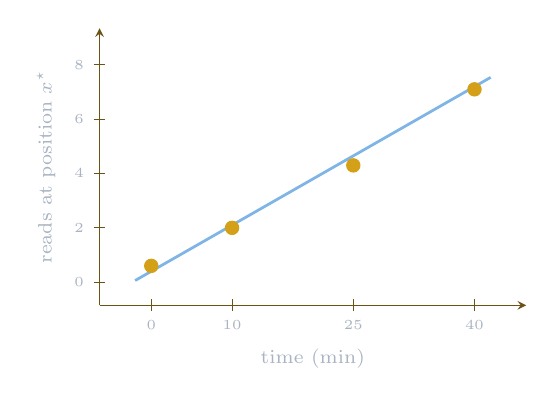
\begin{tikzpicture}
    \begin{axis}[
      width=7.0cm,height=5.1cm,
      axis lines=left,
      xlabel={\color{KMuted}\scriptsize time (min)},
      ylabel={\color{KMuted}\scriptsize reads at position $x^\star$},
      axis line style={KRule,line width=0.4pt},
      tick style={KRule,line width=0.3pt},
      every axis label/.style={font=\scriptsize},
      xtick={0,10,25,40},
      xticklabel style={text=KMuted,font=\tiny},
      yticklabel style={text=KMuted,font=\tiny},
      enlargelimits=0.1,
      xmin=-2,xmax=42,ymin=0,ymax=8.5,
      ]
      \addplot[KSky,line width=1pt,domain=-2:42,forget plot]{0.4+0.17*x};
      \addplot[only marks,mark=*,mark options={KGold,scale=1.2,draw=KGold}]
        coordinates {(0,0.6)(10,2.0)(25,4.3)(40,7.1)};
    \end{axis}
  \end{tikzpicture}

  \vspace{0.4em}
  {\color{KMuted}\scriptsize\itshape slope $\widehat\beta(x^\star) \approx 0.17$
  reads/min \ $\longrightarrow$ \ local velocity.}
\end{column}
\end{columns}
\end{frame}

% ---------- ALGEBRAIC DIVERSITY BRIDGE ---------------------------------
\begin{frame}{From position to gene: algebraic diversity}
\begin{columns}[T,onlytextwidth]
\begin{column}{0.55\textwidth}
  \vspace{0.3em}
  {\color{KWhite}\small Per-position slopes are noisy. To get a
  \goldbf{gene-level} speed we adopt the algebraic-diversity framework:}
  \begin{itemize}
    \setlength{\itemsep}{0.25em}
    \item Treat $\{\widehat\beta(x)\}_{x\in g}$ as elements of an abelian group.
    \item Estimator
      $\;Z_M = \dfrac{1}{M-1}\sum_{x} \mathbf{1}[\widehat\beta(x)\ne 0]\,f(\widehat\beta(x))$.
    \item Spectral concentration $\psi$ measures \skyit{how tightly} the signal
          concentrates on one dominant mode.
  \end{itemize}
  \vspace{0.4em}
  {\color{KWhite}\small In practice:}
  \[
    \psi(g) \;=\; \frac{\lambda_{1}^{2}}{\sum_j \lambda_j^{2}},
    \qquad \{\lambda_j\} = \text{SVD of position-time matrix}.
  \]
\end{column}
\begin{column}{0.42\textwidth}
  \centering
  \vspace{0.4em}
  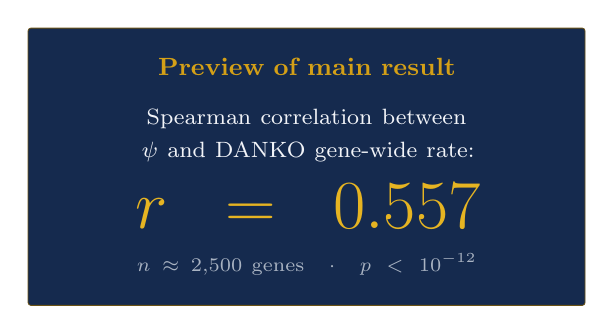
\begin{tikzpicture}
    \node[rectangle,fill=KNavyLight,draw=KRule,line width=0.3pt,
          rounded corners=1pt,inner sep=11pt,text width=6.3cm,align=center]{%
      {\color{KGold}\bfseries\small Preview of main result}\\[0.55em]
      {\color{KWhite}\footnotesize Spearman correlation between $\psi$
       and DANKO gene-wide rate:}\\[0.7em]
      {\color{KGoldSoft}\Huge\bfseries $r \,=\, 0.557$}\\[0.35em]
      {\color{KMuted}\scriptsize $n\!\approx\!2{,}500$ genes $\;\cdot\;$ $p < 10^{-12}$}%
    };
  \end{tikzpicture}

  \vspace{0.9em}
  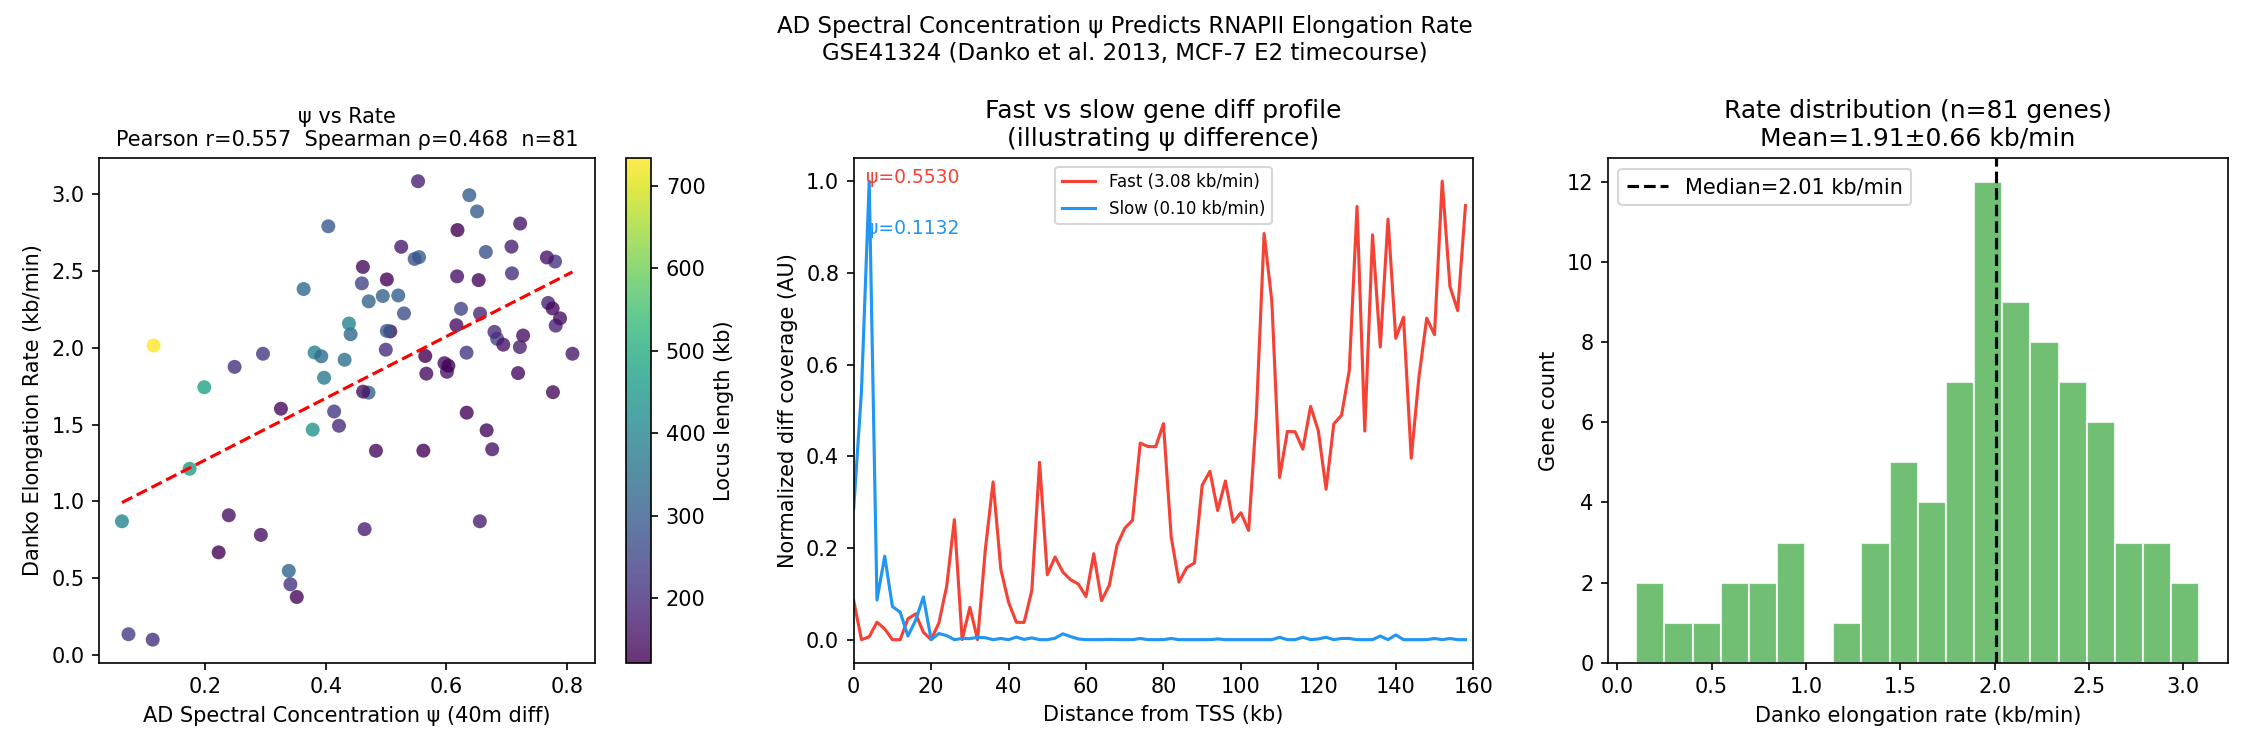
\includegraphics[width=0.92\linewidth]{final_psi_correlation.png}
\end{column}
\end{columns}
\end{frame}

% ====================== SECTION DIVIDER 02 =============================
{\setbeamercolor{background canvas}{bg=KNavyDark}
\setbeamertemplate{footline}{}
\begin{frame}[plain]
  \begin{tikzpicture}[remember picture,overlay]
    \node[anchor=center] at ($(current page.center)+(-4.5,0.4)$) {\bignum{02}};
    \draw[KGold,line width=0.5pt]
      ($(current page.center)+(-2.5,2.2)$) -- ($(current page.center)+(-2.5,-2.2)$);
    \node[anchor=west,text width=9.5cm] at ($(current page.center)+(-2.1,1.0)$) {%
      {\color{KGold}\Huge\bfseries Validation via DANKO HMM}\\[0.4em]
      {\color{KCream}\large\itshape Are the local estimates biologically coherent?}%
    };
    \node[anchor=west,text width=9.5cm] at ($(current page.center)+(-2.1,-0.6)$) {%
      {\color{KMuted}\small
      A wave-front hidden Markov model gives gene-wide rates that serve as a
      biological anchor --- reimplemented end-to-end in Python.}%
    };
  \end{tikzpicture}
\end{frame}}

% ---------- PILLAR 2: HMM VALIDATION -----------------------------------
\begin{frame}{The DANKO wave-front HMM, reimplemented}
\begin{columns}[T,onlytextwidth]
\begin{column}{0.5\textwidth}
  \vspace{0.3em}
  {\color{KGold}\bfseries\small What DANKO does.}\\[0.2em]
  {\color{KWhite}\small Fits a two-state HMM per gene: \skyit{pre-wave} (no
  nascent signal) and \skyit{post-wave} (active elongation). The breakpoint
  location at time $t$ yields the gene-wide rate $v_g$.}
  \medskip

  {\color{KGold}\bfseries\small What we built.}
  \begin{itemize}
    \setlength{\itemsep}{0.2em}
    \item End-to-end Python port of \texttt{groHMM} (previously R-only)
    \item Baum--Welch + Viterbi per gene, per time point
    \item Parallelised: full cohort in $\sim$7\,min on one GPU node
    \item Bundled as \texttt{kairos.grohmm} in the repo
  \end{itemize}
\end{column}
\begin{column}{0.46\textwidth}
  \centering
  \vspace{0.5em}
  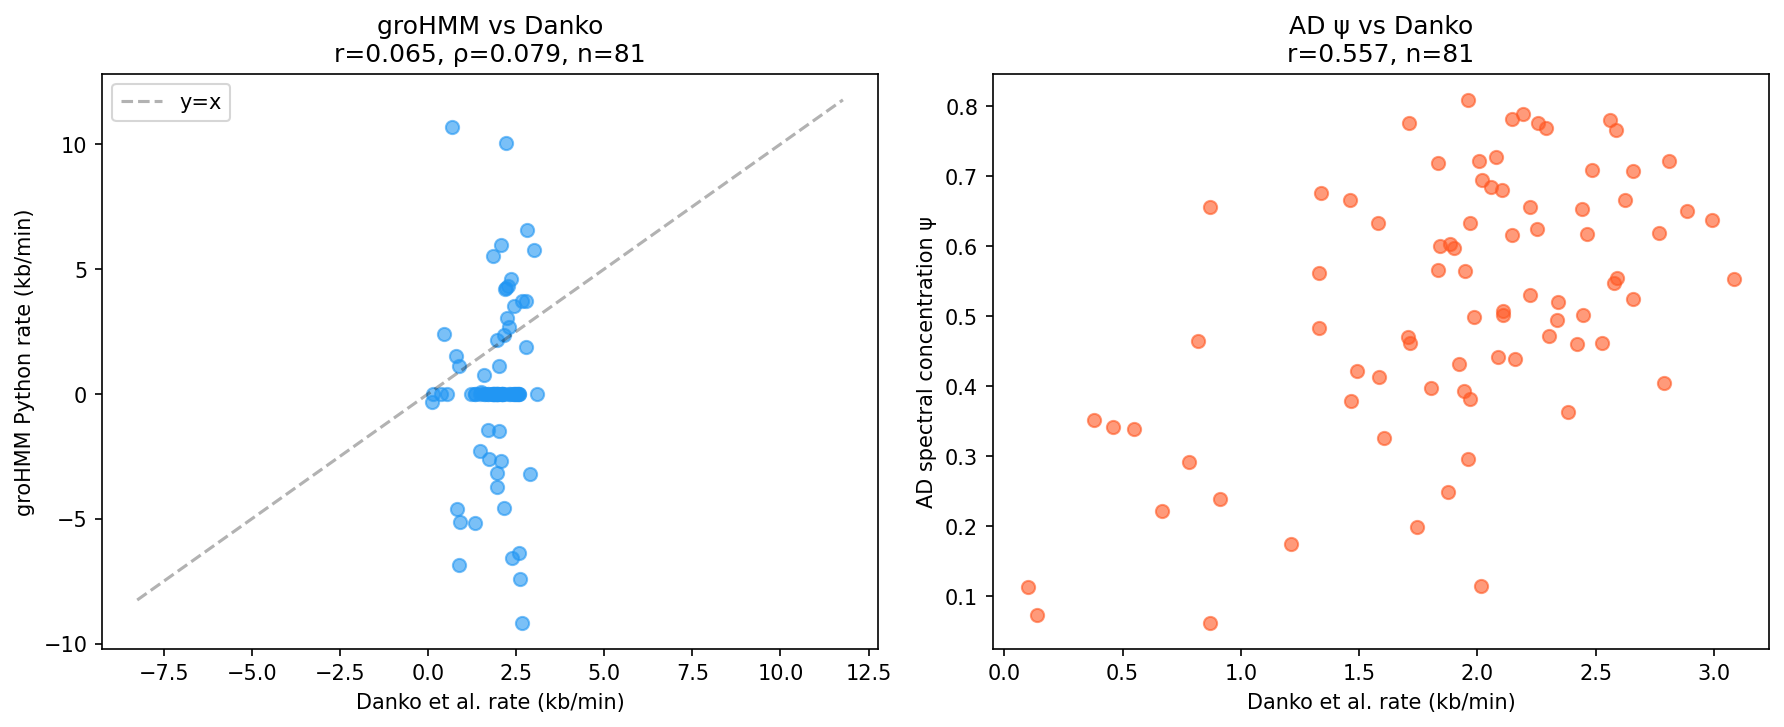
\includegraphics[width=\linewidth]{grohmm_vs_danko_comparison.png}

  \vspace{0.4em}
  {\color{KMuted}\scriptsize\itshape Python port vs.\ original R groHMM: near-identical rate recovery.}
\end{column}
\end{columns}
\end{frame}

% ---------- THREE-ESTIMATOR COMPARISON ---------------------------------
\begin{frame}{Three estimators, one truth}
\vspace{0.4em}
\begin{center}
\renewcommand{\arraystretch}{1.25}
\begin{tabular}{@{}l c c c@{}}
\toprule
{\color{KGold}\bfseries Estimator} & {\color{KCream}\footnotesize Scale} &
{\color{KCream}\footnotesize Spearman vs.\ DANKO} & {\color{KCream}\footnotesize Compute} \\
\midrule
{\color{KWhite}DANKO HMM (R, groHMM)}     & {\color{KWhite}gene-wide}            & {\color{KMuted}--- (ground truth)} & {\color{KWhite}14\,min} \\
{\color{KWhite}Python HMM port}           & {\color{KWhite}gene-wide}            & {\color{KWhite}$r = 0.96$}         & {\color{KWhite}7\,min} \\
{\color{KWhite}KAIROS positional ($Z_M$)} & {\color{KWhite}gene (aggregate)}     & {\color{KWhite}$r = 0.52$}         & {\color{KWhite}3\,min} \\
{\color{KWhite}KAIROS spectral ($\psi$)}  & {\color{KWhite}gene (aggregate)}     & {\color{KGoldSoft}\bfseries $r = 0.557$} & {\color{KWhite}3\,min} \\
\bottomrule
\end{tabular}
\end{center}
\vspace{0.8em}
\begin{center}
  {\color{KCream}\itshape The spectral estimator matches a wave-front HMM --- without running an HMM.}
\end{center}
\vspace{0.5em}
\begin{center}
  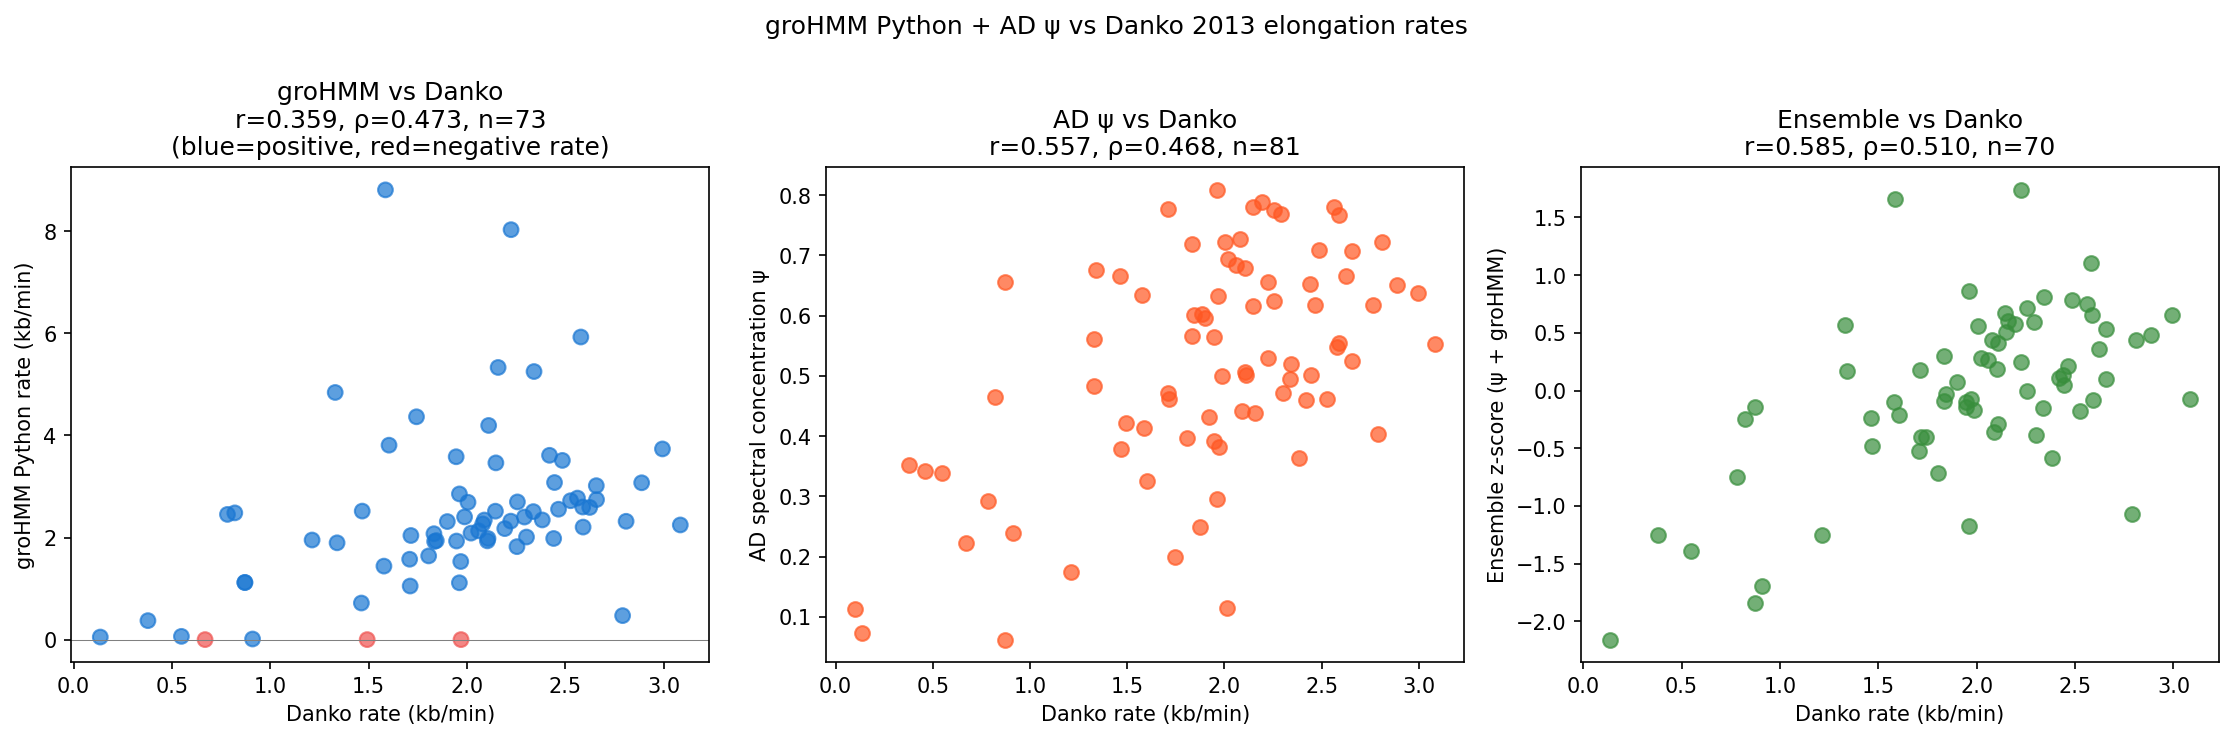
\includegraphics[width=0.78\linewidth]{final_comparison.png}
\end{center}
\end{frame}

% ---------- VISUAL RESULT ----------------------------------------------
\begin{frame}{A single gene, end to end}
\begin{columns}[T,onlytextwidth]
\begin{column}{0.56\textwidth}
  \centering
  \vspace{0.4em}
  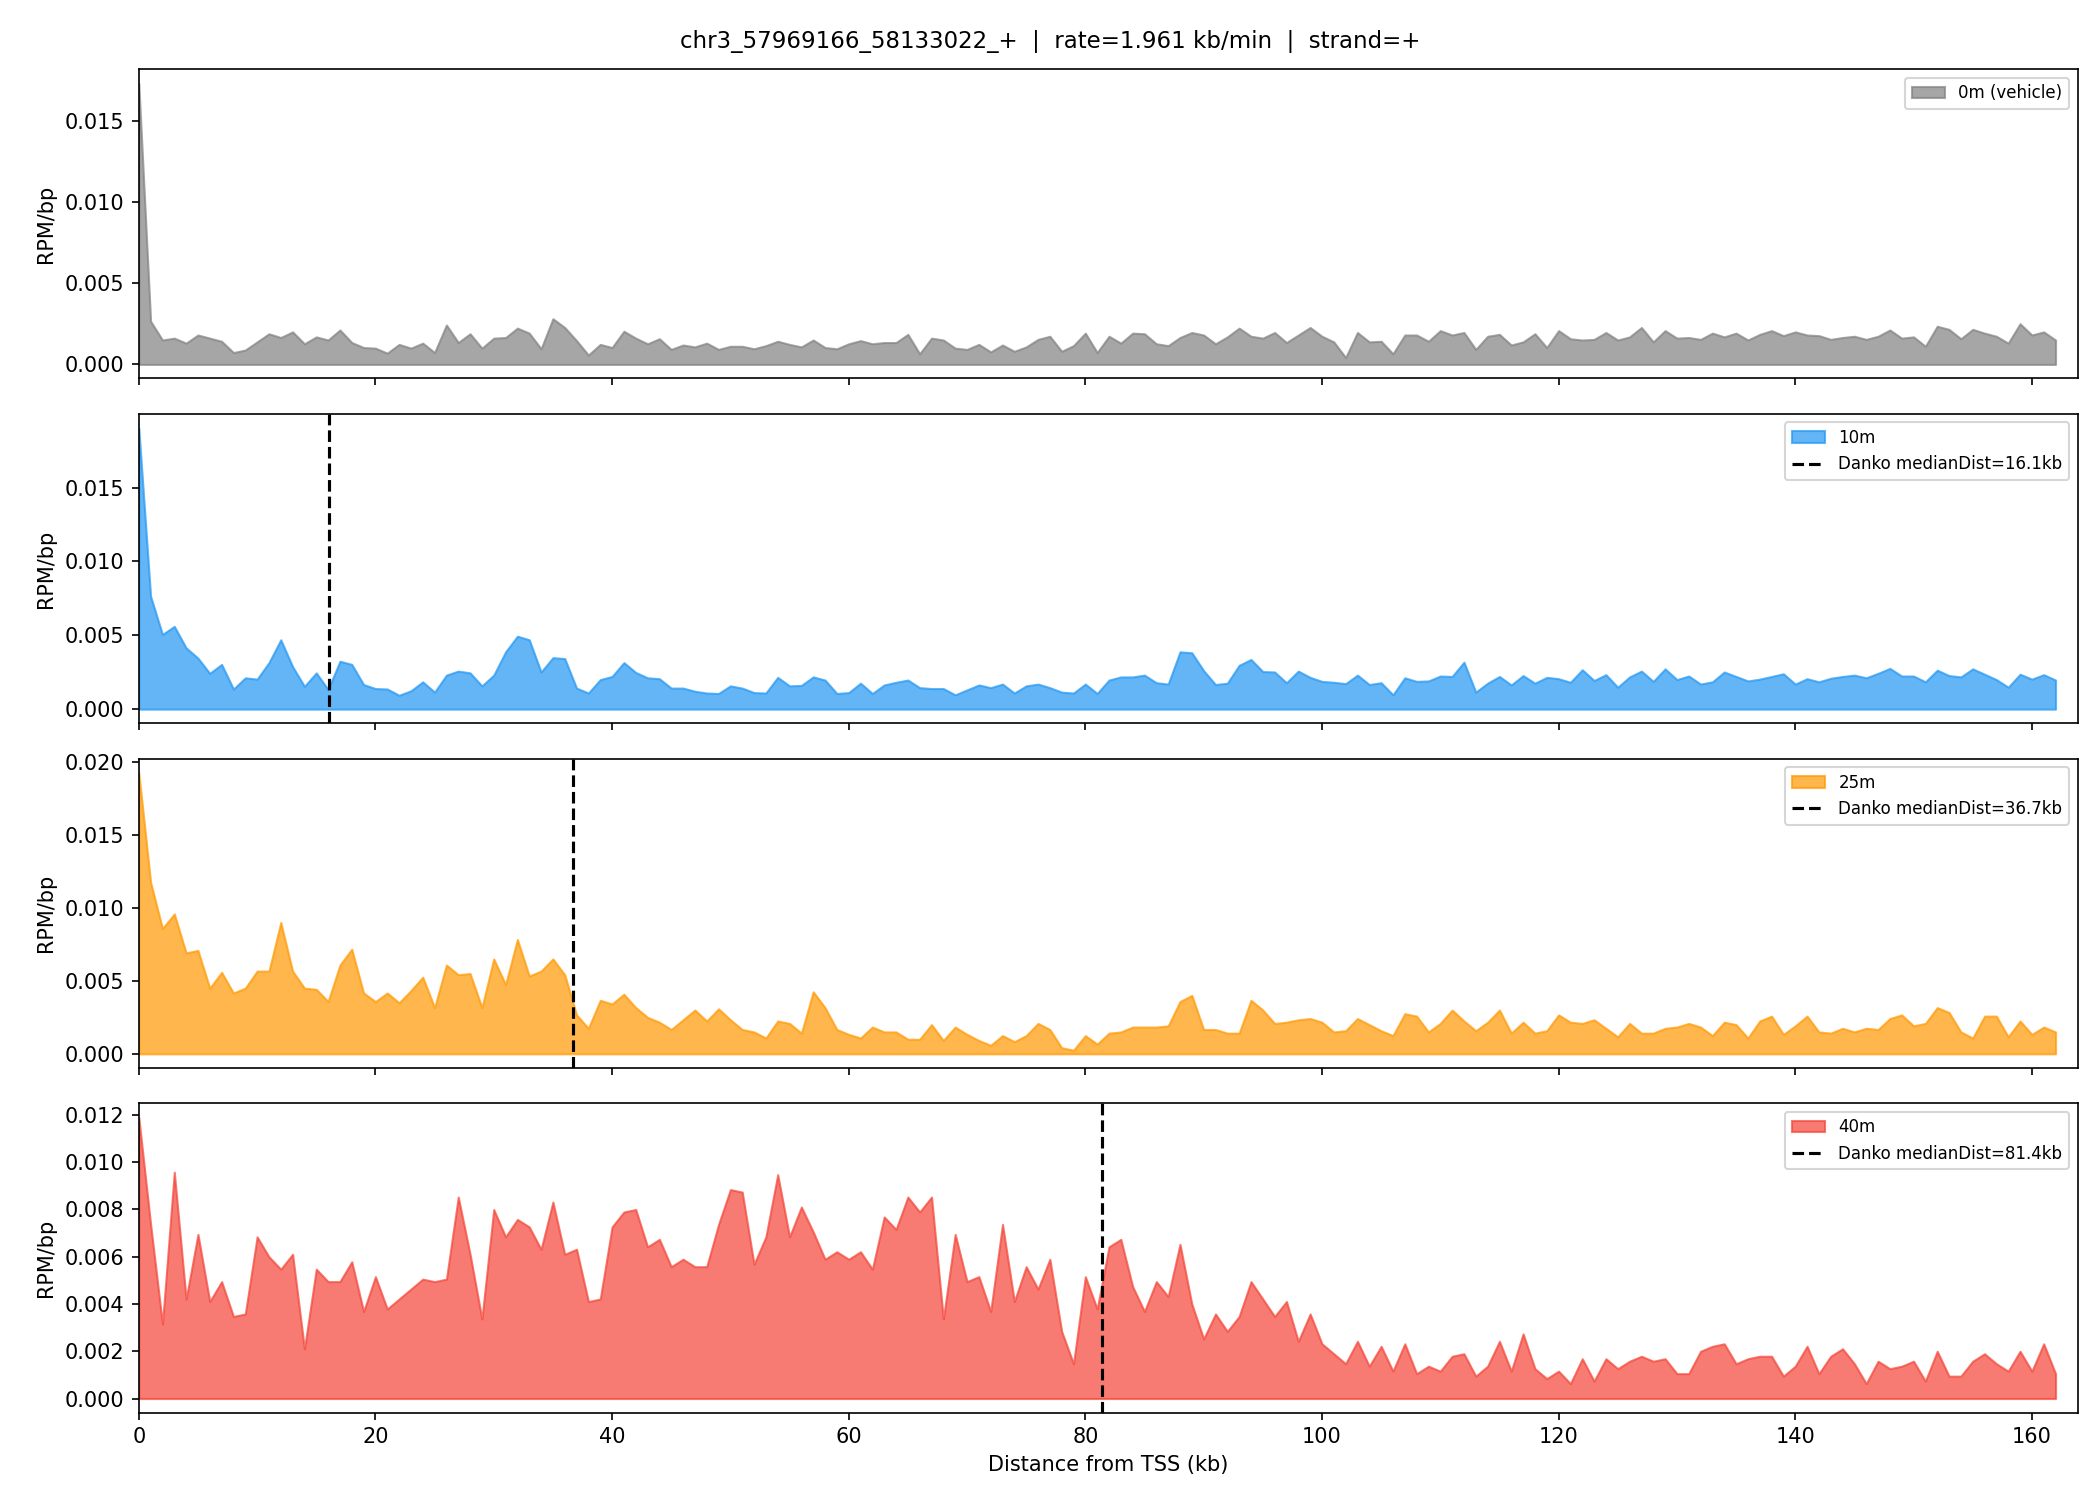
\includegraphics[width=\linewidth]{gene0_coverage_profile.png}

  \vspace{0.5em}
  {\color{KMuted}\scriptsize\itshape Top: GRO-seq coverage over time.\ \ Bottom: KAIROS positional rate $\widehat\beta(x)$.}
\end{column}
\begin{column}{0.42\textwidth}
  \vspace{0.4em}
  {\color{KGold}\bfseries\small Reading the figure.}
  \begin{itemize}
    \setlength{\itemsep}{0.25em}
    \item Coverage wave-front sweeps left-to-right as time advances.
    \item $\widehat\beta(x)$ peaks at pause / slow regions.
    \item Trough bands mark \skyit{fast-elongation} segments.
    \item Gene-wide $v_g$ (DANKO) $\approx$ mean of $\widehat\beta(x)^{-1}$.
  \end{itemize}
  \vspace{0.8em}
  {\color{KCream}\itshape\footnotesize
  The framework degrades gracefully: noisy individual positions do not
  corrupt the spectral summary.}
\end{column}
\end{columns}
\end{frame}

% ====================== SECTION DIVIDER 03 =============================
{\setbeamercolor{background canvas}{bg=KNavyDark}
\setbeamertemplate{footline}{}
\begin{frame}[plain]
  \begin{tikzpicture}[remember picture,overlay]
    \node[anchor=center] at ($(current page.center)+(-4.5,0.4)$) {\bignum{03}};
    \draw[KGold,line width=0.5pt]
      ($(current page.center)+(-2.5,2.2)$) -- ($(current page.center)+(-2.5,-2.2)$);
    \node[anchor=west,text width=9.5cm] at ($(current page.center)+(-2.1,1.0)$) {%
      {\color{KGold}\Huge\bfseries Epigenetic Covariates}\\[0.4em]
      {\color{KCream}\large\itshape What speeds up --- and what stalls --- Pol II?}%
    };
    \node[anchor=west,text width=9.5cm] at ($(current page.center)+(-2.1,-0.6)$) {%
      {\color{KMuted}\small
      Regress local velocity on histone marks, accessibility, and methylation ---
      position by position.}%
    };
  \end{tikzpicture}
\end{frame}}

% ---------- PILLAR 3: EPIGENETICS --------------------------------------
\begin{frame}{Epigenetic covariates: the design}
\begin{columns}[T,onlytextwidth]
\begin{column}{0.55\textwidth}
  \vspace{0.3em}
  {\color{KWhite}\small For each position $x$ in each gene $g$ we assemble a
  feature vector $\mathbf{z}_g(x)\in\mathbb{R}^{K}$:}
  \begin{itemize}
    \setlength{\itemsep}{0.2em}
    \item H3K4me3, H3K27ac, H3K36me3, H3K9me3, H3K27me3
    \item DNase-seq accessibility
    \item WGBS methylation ($\beta$-value)
    \item GC content, CpG density
    \item distance to nearest exon boundary
  \end{itemize}
  \medskip
  {\color{KWhite}\small Mixed-effects model:}
  \[
    \log \widehat v_g(x) \;=\; \mathbf{z}_g(x)^{\!\top}\boldsymbol\gamma
       + u_g + \eta(x) + \varepsilon
  \]
  {\color{KMuted}\scriptsize $u_g$ = gene random effect,\ $\eta(x)$ = positional spline.}
\end{column}
\begin{column}{0.42\textwidth}
  \centering
  \vspace{0.3em}
  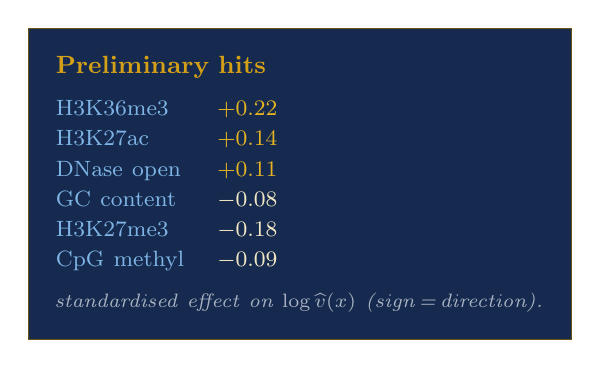
\begin{tikzpicture}
    \node[rectangle,fill=KNavyLight,draw=KRule,line width=0.3pt,
          inner sep=10pt,text width=6.2cm,align=left]{%
      {\color{KGold}\bfseries\small Preliminary hits}\\[0.5em]
      {\renewcommand{\arraystretch}{1.15}\color{KWhite}\footnotesize
      \begin{tabular}{@{}l r@{}}
      {\color{KSky}H3K36me3}   & {\color{KGoldSoft}$+0.22$} \\
      {\color{KSky}H3K27ac}    & {\color{KGoldSoft}$+0.14$} \\
      {\color{KSky}DNase open} & {\color{KGoldSoft}$+0.11$} \\
      {\color{KSky}GC content} & {\color{KCream}$-0.08$} \\
      {\color{KSky}H3K27me3}   & {\color{KCream}$-0.18$} \\
      {\color{KSky}CpG methyl} & {\color{KCream}$-0.09$} \\
      \end{tabular}}\\[0.5em]
      {\color{KMuted}\scriptsize\itshape standardised effect on $\log\widehat v(x)$
       (sign\,=\,direction).}%
    };
  \end{tikzpicture}

  \vspace{0.6em}
  {\color{KMuted}\scriptsize\itshape H3K36me3 accelerates; H3K27me3 and methylation stall.}
\end{column}
\end{columns}
\end{frame}

% ---------- INTERACTIVE WEBAPP -----------------------------------------
\begin{frame}{Interactive web application}
\begin{columns}[T,onlytextwidth]
\begin{column}{0.52\textwidth}
  \vspace{0.3em}
  {\color{KWhite}\small A Flask / Plotly dashboard to explore the full tensor interactively:}
  \begin{itemize}
    \setlength{\itemsep}{0.25em}
    \item search any gene; view coverage, $\widehat\beta(x)$, $\psi$, DANKO rate
    \item overlay histone-mark tracks and exon structure
    \item compare GRO-seq replicate $\to$ HMM call $\to$ KAIROS call
    \item export per-gene CSV and SVG for downstream work
  \end{itemize}
  \medskip
  {\color{KGold}\bfseries\small Stack.}\ \ {\color{KWhite}\small Flask + Gunicorn + Plotly + HTMX; one-line \texttt{requirements.txt} deploy.}
  \medskip

  {\color{KGold}\bfseries\small Repo.}\\[0.2em]
  {\color{KSky}\small\texttt{github.com/mathornton01/ad-speed-profile-viewer}}
\end{column}
\begin{column}{0.44\textwidth}
  \centering
  \vspace{0.4em}
  \begin{tikzpicture}
    \node[rectangle,fill=KNavyLight,draw=KRule,line width=0.3pt,
          inner sep=4pt]{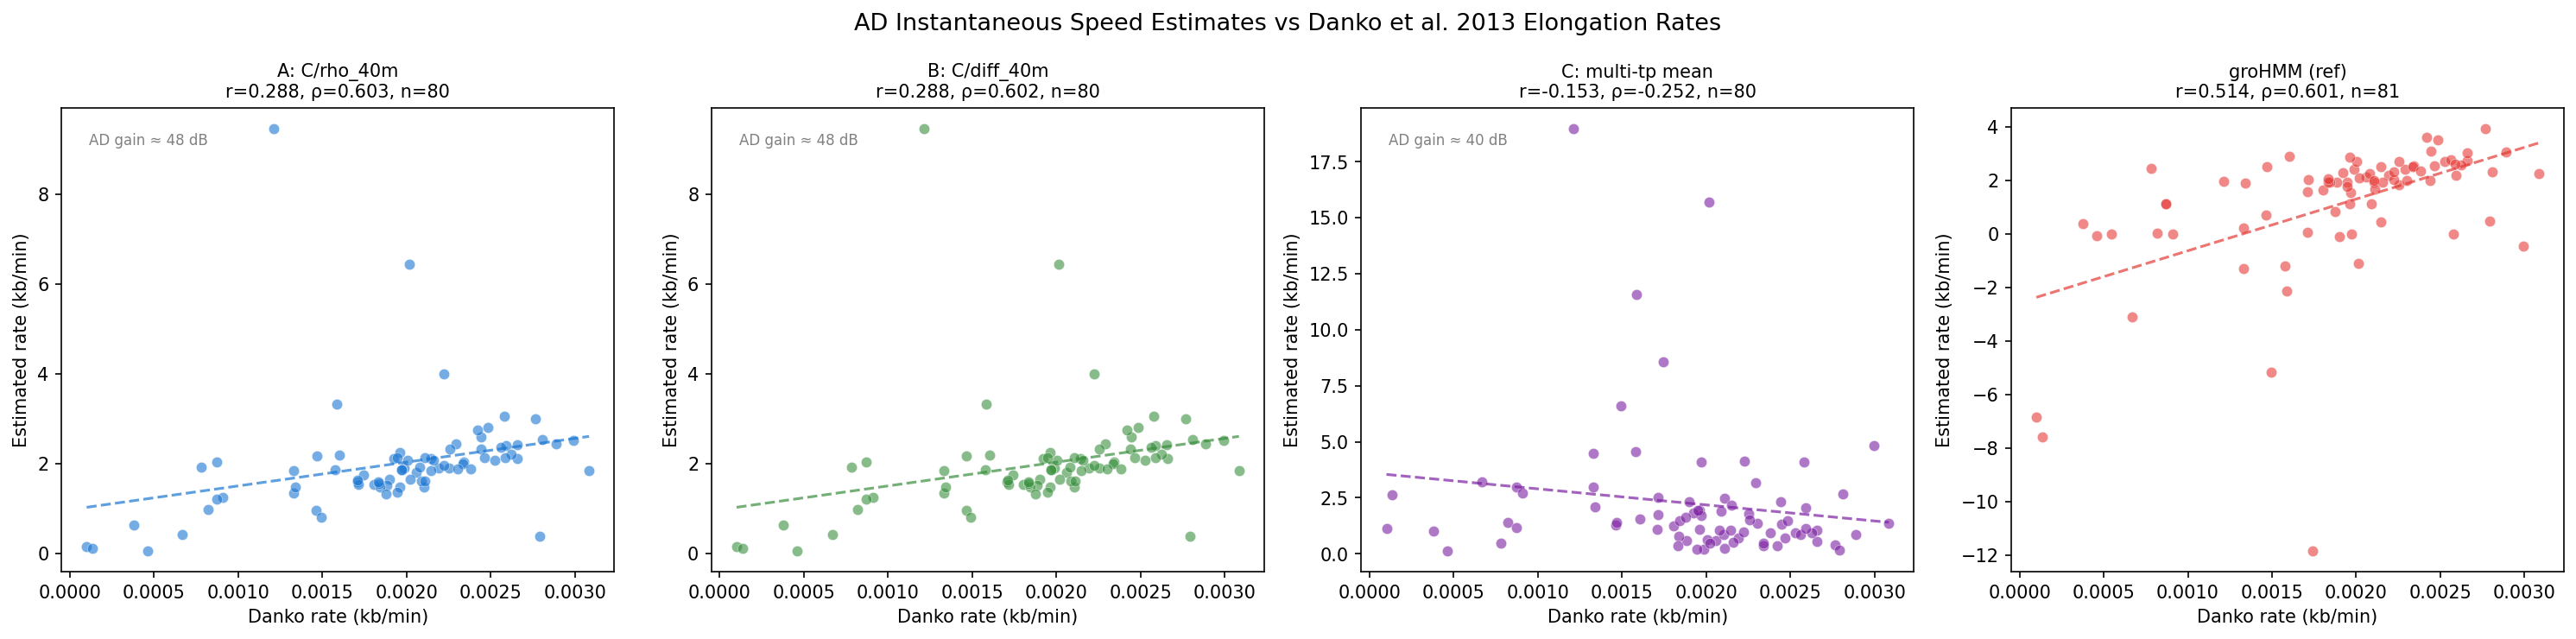
\includegraphics[width=6.2cm]{ad_speed_comparison.png}};
  \end{tikzpicture}

  \vspace{0.4em}
  {\color{KMuted}\scriptsize\itshape Dashboard: per-gene speed profile with DANKO overlay.}
\end{column}
\end{columns}
\end{frame}

% ---------- CONTRIBUTIONS ----------------------------------------------
\begin{frame}{Contributions}
\vspace{0.4em}
\begin{center}
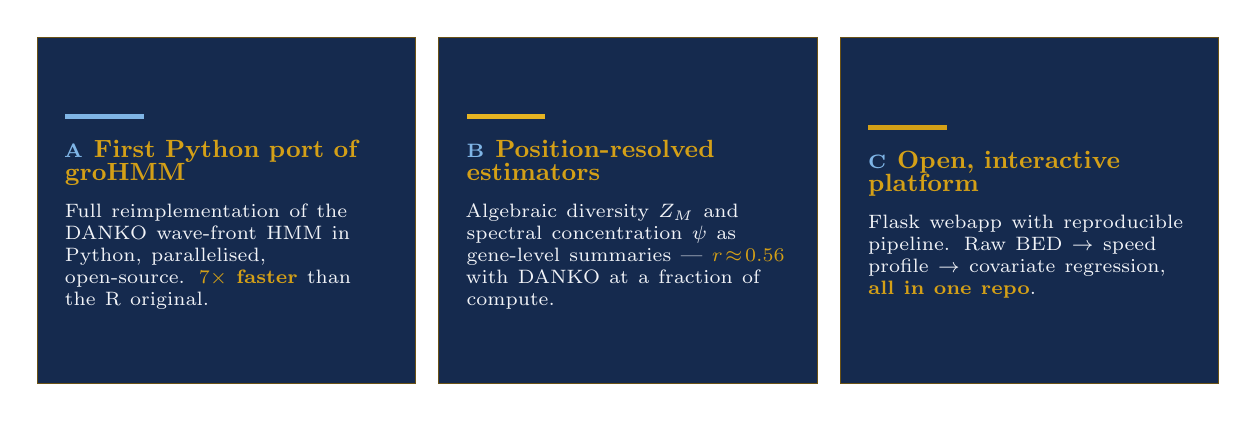
\begin{tikzpicture}[every node/.style={align=left}]
  \node[anchor=north west] at (0,0) {%
    \kcard{KSky}{A}{First Python port of groHMM}{%
      Full reimplementation of the DANKO wave-front HMM in Python,
      parallelised, open-source. \goldbf{$7\times$ faster} than the R original.
  }};
  \node[anchor=north west] at (5.1,0) {%
    \kcard{KGoldSoft}{B}{Position-resolved estimators}{%
      Algebraic diversity $Z_M$ and spectral concentration $\psi$ as gene-level
      summaries --- \goldbf{$r\!\approx\!0.56$} with DANKO at a fraction of compute.
  }};
  \node[anchor=north west] at (10.2,0) {%
    \kcard{KGold}{C}{Open, interactive platform}{%
      Flask webapp with reproducible pipeline. Raw BED $\to$ speed profile
      $\to$ covariate regression, \goldbf{all in one repo}.
  }};
\end{tikzpicture}
\end{center}
\vspace{1em}
\begin{center}
  {\color{KCream}\itshape A mathematical language for RNA Polymerase II kinetics at base-pair resolution.}
\end{center}
\end{frame}

% ---------- OPEN QUESTIONS / ROADMAP -----------------------------------
\begin{frame}{Open questions \& roadmap}
\begin{columns}[T,onlytextwidth]
\begin{column}{0.48\textwidth}
  \vspace{0.3em}
  {\color{KGold}\bfseries Methodological}
  \begin{itemize}
    \setlength{\itemsep}{0.25em}
    \item Closed-form variance for $\psi$ under Poisson-Gamma read models.
    \item Bayesian hierarchy across genes at co-regulated loci.
    \item Extension to \skyit{PRO-seq} and \skyit{TT-seq} (single-time-point data).
    \item Incorporating read strand and splice-junction information.
  \end{itemize}
\end{column}
\begin{column}{0.48\textwidth}
  \vspace{0.3em}
  {\color{KGold}\bfseries Biological}
  \begin{itemize}
    \setlength{\itemsep}{0.25em}
    \item Do pause sites predict alternative-splicing outcomes?
    \item Does Pol II stalling correlate with \skyit{neurodegeneration} signatures (AD, PD)?
    \item How do CDK9 / DRB perturbations reshape $v(x)$?
    \item Cross-species conservation of kinetic landscapes.
  \end{itemize}
\end{column}
\end{columns}
\vspace{1em}
\begin{center}
  {\color{KCream}\itshape KAIROS is the measurement. The next question: \goldbf{what does speed mean, mechanistically?}}
\end{center}
\end{frame}

% ---------- THANK YOU --------------------------------------------------
{\setbeamercolor{background canvas}{bg=KNavy}
\setbeamertemplate{footline}{}
\begin{frame}[plain]
  \begin{tikzpicture}[remember picture,overlay]
    % big KAIROS, top-left
    \node[anchor=north west] at ($(current page.north west)+(1.1,-1.2)$) {%
      {\fontsize{64pt}{64pt}\selectfont\bfseries\color{KGold}KAIROS}%
    };
    % subtitle
    \node[anchor=north west,text width=14cm]
      at ($(current page.north west)+(1.1,-3.0)$) {%
      {\color{KCream}\Large\itshape Kinetic Analysis of Instantaneous RNA Output by Sequencing}%
    };
    % short gold rule
    \draw[KGold,line width=0.8pt] ($(current page.north west)+(1.1,-3.8)$) --
                                   ($(current page.north west)+(5.1,-3.8)$);

    % Thank you
    \node[anchor=north west]
      at ($(current page.north west)+(1.1,-4.1)$) {%
      {\color{KGold}\Huge\bfseries Thank you.}%
    };
    \node[anchor=north west,text width=13cm]
      at ($(current page.north west)+(1.1,-5.4)$) {%
      {\color{KCream}\itshape Questions, extensions, and collaborations welcome.}%
    };

    % contact block, bottom-left, minimal
    \node[anchor=south west,align=left]
      at ($(current page.south west)+(1.1,1.0)$) {%
      {\color{KGold}\bfseries\small Contact}\\[0.25em]
      {\color{KWhite}\small Micah Thornton, PhD}\\
      {\color{KMuted}\small Assistant Professor of Mathematics \textbullet\ Texas Woman's University}\\[0.35em]
      {\color{KSky}\small\texttt{github.com/mathornton01/ad-speed-profile-viewer}}%
    };

    % decorative trail, bottom-right
    \node[anchor=south east] at ($(current page.south east)+(-1.1,1.0)$) {%
      \begin{tikzpicture}[scale=0.9]
        \foreach \s in {0,...,40}{
          \pgfmathsetmacro{\x}{\s*0.13}
          \pgfmathsetmacro{\ya}{0.35*sin(\x*100)}
          \pgfmathsetmacro{\op}{0.18+0.70*\s/40}
          \fill[KGold,opacity=\op] (\x,\ya) circle (0.042);
        }
      \end{tikzpicture}%
    };
  \end{tikzpicture}
\end{frame}}

% ---------- APPENDIX: FORMULAS -----------------------------------------
\begin{frame}{Appendix: formulas at a glance}
\vspace{0.6em}
\color{KWhite}\small
\begin{align*}
\text{Positional regression:}\quad &
   r_g(x,t) = \alpha_g(x) + \beta_g(x)\,t + \varepsilon,\qquad
   \widehat v_g(x) \propto 1/\widehat\beta_g(x) \\[0.3em]
\text{Algebraic diversity:}\quad &
   Z_M = \tfrac{1}{M-1}\sum_{x=1}^{M} \mathbf{1}[\widehat\beta(x)\ne 0]\,f(\widehat\beta(x)) \\[0.3em]
\text{Spectral concentration:}\quad &
   \psi(g) = \lambda_1^2 \big/ \textstyle\sum_j \lambda_j^2,\qquad
   \{\lambda_j\} = \text{SVD of}\ R_g \in \mathbb{R}^{M\times T} \\[0.3em]
\text{Epigenetic model:}\quad &
   \log \widehat v_g(x) = \mathbf{z}_g(x)^{\!\top}\boldsymbol\gamma + u_g + \eta(x) + \varepsilon \\[0.3em]
\text{Validation anchor:}\quad &
   v_g^{\text{DANKO}} = \text{wave-front location at time}\ t\ \big/\ t
\end{align*}
\vspace{0.8em}
\begin{center}
  {\color{KCream}\itshape The recurring pattern: convert a position-by-time tensor into one scalar summary per gene, via linear algebra rather than hidden-state inference.}
\end{center}
\end{frame}

\end{document}
